\section{Linear Algebra}
\subsection{Linear Transformations}
\begin{definition}[Linear Transformation]
	Let $V\in\R^d$ and $W\in\R^m$ be two vectors spaces. A function $T:V\rightarrow W$ is called a linear transformation of $V$ into $W$, if $\forall u, v \in V$ and $c\in \R$.
	\begin{itemize}
		\item Additivity: $T\left(u+v\right) = T\left(u\right)+T\left(v\right)$
		\item Scalar multiplication: $T \left(cu\right) = cT \left(u\right)$
	\end{itemize}
\end{definition}

~\\
For $V$  and $W$ of a finite dimension, any linear transformation can be represented by a matrix $A$. Therefore, from now and on we will focus only on finite-dimensional spaces, and implicitly refer to the matrix representing the linear transformation.


\begin{definition}[Affine Transformation]
	An \textit{affine transformation} is a transformation of the form $T\left(u\right)=Au+w,$ where $u\in V, w\in W$.
\end{definition}

Notice, that by definition an affine transformation is not a linear transformation. Notice that for a linear transformation $A$ it holds that $A\cdot 0_V = 0_W$, but in the case of an affine transformation where $0\neq w\in W$ then $T\left(0_V\right)=A\cdot 0_V + w \neq 0_w$.


~\\Let us define some vector spaces associated with each linear transformation
\begin{definition}
Let $A$ be the matrix corresponding the linear transformation $T:V\rightarrow W$. We define the:
\begin{itemize}
	\item Kernel- (or null-) space of $A$ as $Ker\left(A\right)\coloneqq\left\{x\in V|Ax=0\right\}$. Also denotes as $N\left(A\right)$.
	\item Image- (or column-) space of $A$ as $Im\left(A\right)\coloneqq\left\{w\in W|w=Ax,x\in V\right\}$. Also denotes as $Col\left(A\right)$.
	\item Row space of $A$ as $Im\left(A^\top\right)\coloneqq\left\{x\in V|x=A^\top w,w\in W\right\}$. Equivelantly it can be defined as the column space of $A^\top$ and therefore denoted as $Col\left(A^\top\right)$.
	\item Null space of $A^\top$ as $Ker\left(A^\top\right)\coloneqq \left\{x\in W | A^\top x = 0\right\}$. This space is also referred to as the left null space of $A$.
\end{itemize}
\end{definition}

Note that by definition, $Ker\left(A\right), Row\left(A\right)\subseteq V$ and $Im\left(A\right)\subseteq W$. Using the above definitions let us gain some insights into what these vector spaces provide us with.\\

\begin{definition}
Let $A\in\R^{m\times d}$. The rank of $A$ is the maximum number of linearly independent rows of $A$ and denoted by $rank\left(A\right)$.
\end{definition}

It holds that the rank of $A$ equals both the dimension of the columns space and of the row space of $A$. As such, we refer to $A$ being of \textit{full rank} if and only if $rank\left(A\right)=min\left(m,d\right)$. Otherwise we say that $A$ is rank deficient.\\

\begin{definition}
Let $A\in\R^{d\times d}$ be a square matrix. $A$ is called  invertible (or non-singular) if there exists a matrix $B\in\R^{d\times d}$ such that $AB=I_d=BA$. We denote the inverse by $A^{-1}$.
\end{definition}

\begin{claim}
Let $A$ be a square matrix. The following are equivalent (TFAE):
\begin{itemize}
	\item $A$ is invertible (non-singular)
	\item $A$ is full-rank
	\item $Det\left(A\right)\neq 0$
	\item $Im\left(A\right)=\R^m$ (i.e., the image is the whole space)
	\item $ker\left(A\right)=\vec 0$
\end{itemize}
\end{claim}

~\\
\begin{example}
Consider the following scenario: Suppose we are given a set of $n$ linearly independent linear equations, each of the form $y_i=\sum_{j=1}^{d}\w_j\cdot x_{ij}$, where the $x_{i,j}$'s and $y_i$ are given while $\w_j$'s are unknown. We would like to find a solution for this system of equations. That is, a coefficients vector $\w\in\R^d$ that satisfies:
$$ \forall i\in[d] \,\,\, y_i=\sum_{j=1}^d \w_j \cdot x_{ij} = \w^\top x_i$$
~\\
Let us rearrange the equations in matrix form. Given a linear equation we will denote all it's $x$'s by the vector $x_i\in\R^d$ where $i$ denotes the numbering of the current equation. Similarly we will arrange all the $y$'s in a vector $y\in\R^m$. Thus, we can represent the problem written above as follows:
$$  \text{Find}  \,\,\,\w\in\R^d \,\,\, \text{such that}\,\,\, y=X\w$$
~\\
As we assumed that all linear equations are independent, the rows of $X$ are linearly independent. Therefore, it is of full rank and there exists an invertible matrix $X^{-1}$ such that $XX^{-1}=I$. Equipped with this observation finding $\w$ is simply:
$$ y=X\w \,\, \Rightarrow \,\, X^{-1}y=X^{-1}X\w \,\, \Rightarrow \\, \w=X^{-1}y$$
\end{example}

\begin{remark}
Let us think of each vector $x_i\in\R^d$ as some independent observation (or sample) we have of some phenomena. Each coordinate of $x_i$ corresponds some measurement we have of this observation. Together with this sample we are given some response value $y_i\in\R$. By solving for $\w$ we learn the relation between the $x$'s and $y$'s. Now suppose we are given a new sample $x\in\R^d$. As we already know the relation between the $x$s and the $y$s, we can predict what is the appropriate $y$ value it achieves.
~\\
The general problem of finding such vectors is called \textbf{Regression}. In the case where the relationship is linear it is called \textbf{Linear Regression}. We will discuss linear regression in \autoref{chp:lin_reg}.
\end{remark}

\subsection{Norms, Inner Products and Projections}
More many applications in machine learning we are interested in measuring distances between vectors or sizes of vectors, and "using" a vector (or set of vectors) on another vector. For such, let us formulate these notions.

\begin{definition}[Metric]
A function on a set $X\subseteq \mathbb{F}^k$ $d:X\times X\rightarrow \R_+$ is called a metric function (or distance function) $iff$ for any $v,u,w\in X$ it holds that:
\begin{itemize}
	\item $d\left(v,u\right)=0\iff v=u$
	\item Symmetry: $d\left(v,u\right) = d\left(u,v\right)$
	\item Triangle inequality $d\left(v,u\right) \leq d\left(v,w\right)+d\left(w,u\right)$.
\end{itemize}
\end{definition}
These conditions also imply that a metric is non-negative. As such, we also call a metric function a positive-definite function. Some common metric functions are the absolute distance or the Euclidean distance.

\begin{exercise}
Let $v,u\in\R^k$. Show that the absolute distance, defined as the sum of absolute element-wise subtraction betwen the vectors $d\left(v,u\right)\coloneqq \sum \left|v_i-u_i\right|$, is a metric function.
\end{exercise}
\begin{proof}
Firstly, notice that for some scalars $a,b\in\R$ it holds that $\left|a-b\right|=0$ $iff$ $a=b$. Therefore $d$, being a sum of non-negative elements equals zero $iff$ all elements are zero. This takes place $iff$ $v=u$. Next, symmetry of $d$ is achieved through symmetry of the absolute value function. Lastly, let $v,u,w\in\R^k$ then $$ d\left(v,u\right) = \sum\left|v_i-u_i\right| = \sum\left|v_i - w_i + w_i - u_i\right| \leq \sum\left|v_i-w_i\right| + \sum\left|w_i-u_i\right| = d\left(v,w\right) + d\left(w,u\right) $$
\end{proof}

Next, let us define the notion of a \textit{size} of a vector.
\begin{definition}[Norm] 
	A norm is a function $\norm{\cdot}:\R^d \rightarrow \R_+$ that satisfies the following three conditions for all $a \in \R$ and all $u, v \in \R^d$:
	\begin{itemize}
		\item Positive definite: $\norm{v} \ge 0$ and $\norm{v} = 0$ $iff$ $v$ is the zero vector.
		\item Positive homogeneity: $\norm{av} = \left|a\right|\cdot \norm{v}$.
		\item Triangle inequality: $\norm{v+u} \leq \norm{v} + \norm{u}$.
	\end{itemize}
\end{definition}
We can think of this size in the sense of vector's \textit{distance} from the origin, under some distance function defined by the norm. A few commonly used norms are:
\begin{itemize}
	\item Absolute norm ($\ell_1$): $\norm{v}_1 \coloneqq \sum\left|v_i\right|$.
	\item Euclidean norm ($\ell_2$): $\norm{v}_2 \coloneqq \sqrt{\sum x_i^2}$.
	\item Infinity norm: $\norm{x}_\infty \coloneqq max_i \left|v_i\right|$.
\end{itemize}
\begin{remark}
The absolute and Euclidean norms are part of a wider family of norms called the $L_p$ norms defined as $\norm{v}_p \coloneqq \left(\sum\left|v_i^p\right|\right)^{1/p},\quad p\in\N$.
\end{remark}

\begin{definition}
	Let $V$ be a vector space and $\norm{cdot}$ be a norm over this space. The unit ball of $\norm{\cdot}$ is defined as the set of vectors such that:  $B_{\norm{\cdot}} = \left\{v\in V: \norm{v} \leq 1\right\}.$
\end{definition} 

\begin{figure}[H]
	\centering
	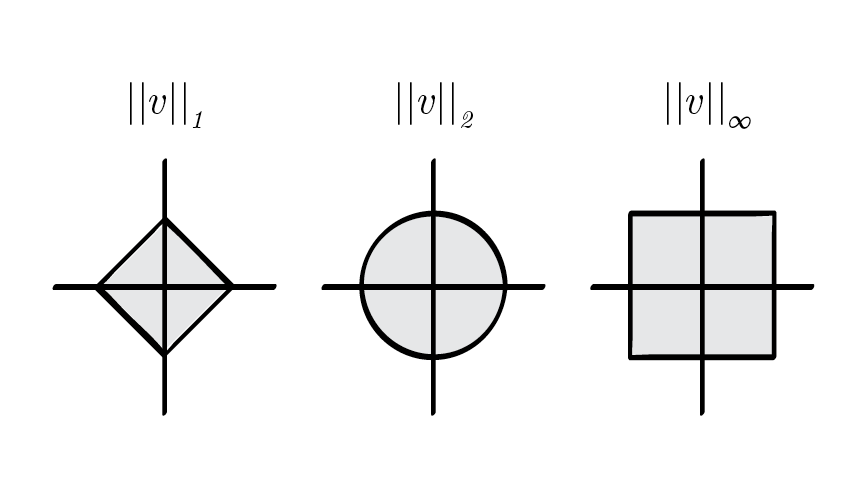
\includegraphics[width=0.6\textwidth]{chapters/mathematical.basis/figures/1_1.png}  
\end{figure}

~\\
Now that we have defined the notions of distances and sizes of vectors, we want to define what it means to ``apply`` some vector on another.

\begin{definition}[Inner Product] 
An inner product space is a vector space $V$ over $\R$ together with a map $\inprod{\cdot}{\cdot}:V\times V\rightarrow\R_+$ satisfying that $\forall v,u,w\in V, \alpha \in\R$:
\begin{itemize}
	\item Symmetry: $\inprod{v}{u}=\inprod{u}{v}$
	\item Linearity: $\inprod{\alpha v+w}{u}=\alpha \inprod{v}{u} + \inprod{w}{u}$
	\item Non-negativity : $\inprod{v}{v}\geq 0$  and $\inprod{v}{v}=0 \iff v=0$ 
\end{itemize}
\end{definition}

Notice the similarity between the definition of a norm and of an inner product. In fact, given an inner-product space, we are also given a norm on this space.

\begin{claim}[Induced Norm] Let $H$ be an inner product space. Then the function $\norm{\cdot}:H\rightarrow \R_+$ is defined $\forall v\in H$ by $\norm{v}=\inprod{v}{v}^{\frac{1}{2}}$ is a norm on $H$.
\end{claim}


\begin{exercise} 
Let $v,u\in V$. Show that  $\inprod{v}{u}=\norm{v}\norm{u}\cos\theta,$ where $\theta$ is the angle between $v,u$.
\end{exercise} 
\begin{proof}
Recall the Law of Cosines:  in a triangle with lengths $a,b,c$, then  $$c^2=a^2+b^2-2ab\cos\theta$$
By applying the cosine law to the triangle defined by $v$ and $u$ and $v-u$ we see that:
$$ \norm{v-u}^2=\norm{v}^2+\norm{u}^2-2\norm{v}\cdot\norm{u}\cdot \cos \theta$$
On the other hand we also know that:
$$ \norm{v-u}^2=\inprod{v-u}{v-u}=\inprod{v}{v}-2\inprod{v}{u}+\inprod{u}{u}= \norm{v}^2+\norm{u}^2-2\inprod{v}{u}$$
Hence, we conclude that: $$\norm{v}\cdot\norm{u}\cdot \cos \theta = \inprod{v}{u}$$
\end{proof}

From the above, we have an expression for the angle between two vectors, using the inner-product. We can therefore define what it means to project one vector onto the other. Using the identity of $\cos\theta$: $$p=\norm{v}\cos\theta\cdot \frac{u}{\norm{u}}=\norm{v}\frac{ \inprod{v}{u}}{\norm{v}\cdot\norm{u}}\cdot \frac{u}{\norm{u}}=\frac{ \inprod{v}{u} }{\norm{u}^2}\cdot u$$
\begin{figure}[H]
	\centering
	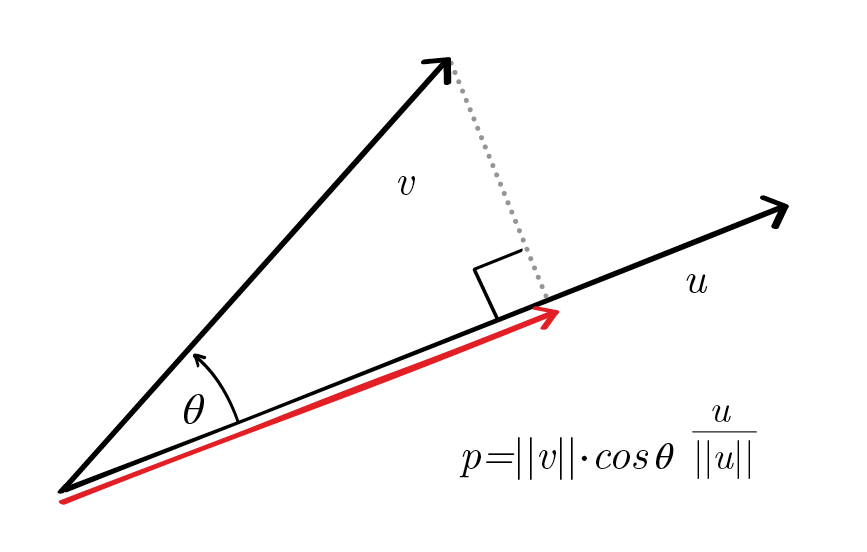
\includegraphics[width=0.5\textwidth]{chapters/mathematical.basis/figures/1_2.png}  
\end{figure}

\begin{definition}[Vector Projection]
A projection of a vector $v$ onto a vector $u$, is a vector $p$ of length $\norm{v} \cos \theta$ in the direction of $u$.
\end{definition}


Notice, that for the special case where $\theta=90^{\circ}$ we get $\inprod{v}{u}=0$. In this case we say that the vectors $v,u$ are ``orthogonal``, and use the notation: $v\bot u$. If $v,u$ are also unit vectors we say that the vectors $v,u$ are ``orthonormal`` to each other.



\begin{definition}
An orthogonal matrix is a square matrix whose columns are unit vectors orthogonal to one another (i.e. they are orthonormal vectors) and whose rows are unit vectors orthogonal to one another.
\end{definition}

\begin{lemma}
Let $A\in \R^{d\times d}$ orthogonal matrix, then $$AA^\top=I=A^\top A$$
\end{lemma}

Putting together the definitions of a vector projection and orthogonal matrices we can define the notion of orthogonal projecting a vector onto some linear subspace.

\begin{definition}

Let $V$ be a $k$-dimensional subspace of $\mathbb{R}^{d}$, and let $v_{1},\ldots,v_{k}$ be an orthonormal basis of $V$. Define $P=\sum_{i=1}^{k}v_{i}v_{i}^{\top}$. The matrix $P$ is an \textbf{\emph{orthogonal projection matrix}}
onto the subspace $V$.
\end{definition}

The following lemma summarizes some useful properties of orthogonal projection matrices.
\begin{lemma}
Let $v_1,\ldots,v_k$ be a set of orthonormal vectors, and let $P=\sum_{i=1}^{k}v_i \otimes  v_i^\top=\sum_{i=1}^{k}v_{i}v_{i}^{\top}$. $P$ has the following properties:
	
\begin{itemize}
	\item $P$ is symmetric
	\item $P^{2}=P$
	\item The eigenvalues of $P$ are either 0 or 1. $v_1,\ldots,v_k$
	are the eigenvectors of $P$ which correspond to the eigenvalue $1$.
	\item $(I-P)P=0$
	\item $\forall x\in\R^d$ and $\forall u\in V$, $\norm{x-u} \geq \norm{x-Px}$
	\item $x\in V\Rightarrow Px=x$
\end{itemize}
\end{lemma}

\begin{remark}
Notice that the definition of the projection matrix includes a sum of \href{https://en.wikipedia.org/wiki/Outer_product}{outer products}
\end{remark}


\subsection{Matrix Decompositions}
Matrix factorizations/decompositions are a strong tool with many theoretical as well as practical usages. It often appears in many different machine learning approaches, some of which we will encounter.

\begin{definition}
Let $A$ be a square matrix. $A$ is diagonalizable if there exists an invertible matrix $P$ such that $P^{-1}AP$ is diagonal.
\end{definition}

Next, we would like to see if we could represent $A$ as the multiplication of orthogonal matrices, and a diagonal one.

\begin{definition}[Eigenvector and Eigenvalue]
Let $A$ a square matrix. We say that a vector $0\neq v\in V$ is an eigenvector of $A$ corresponding to an eigenvalue $\lambda\in\R$ if $Av=\lambda v$.
\end{definition}

\begin{claim}
Let $A$ be a square symmetric matrix. Then there exists an orthonormal basis $u_1,...,u_n\in\R^d$ of eigenvectors of $A$.
\end{claim}

\begin{theorem}[EVD]
Let $A\in \R^{d\times d}$ be a real symmetric matrix. Then there exist an orthonormal matrix $U\in \R^{d\times d}$ and a diagonal matrix $D$ such that, $D_{i,i}$, $i=1..n$ are the eigenvalues of $A$ and $A=UDU^\top$.
\end{theorem}

This decomposition of $A$ is called Eigenvalues Decomposition (EVD). It is widely used and has some strong properties. For example, notice that it is very easy to compute high powers of $A$: $A^k=UDU^\top\cdot UDU^\top\cdot UDU^\top=UD^kU^\top$. It is also very easy to compute the inverse of $A$, if it exists: $A^{-1}=UD^{-1}U^\top$. 

~\\A drawback of the EVD is the restriction to square symmetric matrices. Though this is a rich family of matrices we would like to derive some useful decomposition for non-symmetric and even non-square matrices.

\begin{definition}
Let $\left(V,\norm{\cdot}\right)$ be a normed space. We say that $v\in V$ is a unit vector $iff$ $\norm{v}=1$.
\end{definition}
\begin{definition}
Let $A\in\R^{m\times d}$ and let $v\in\R^d,\, u\in\R^d$ be unit vectors. We say that $v,u$ are right- and left singular vectors of $A$, respectively, corresponding to a singular value $\sigma\in\R_{+}$ if $Av=\sigma u$.
\end{definition}

\begin{theorem}[Singular Value Decoposition (SVD)]
Let $A\in\R^{m\times d}$ be a real matrix. $A$ can be written as a singular value decomposition of the form $A=U\Sigma V^{\top}$, where $U\in \R^{m\times m}$ and $V\in\R^{d\times d}$ are orthonormal  matrices, and $\Sigma\in \R^{m\times d}$ is a diagonal matrix \bf{with non-negative values}. These are called the \textbf{singular values} of $A$.
\end{theorem}
\begin{claim}
Let $A=U\Sigma V^\top$ be an SVD of a matrix $A$. It holds that the columns of $U$ and the rows of $V^\top$ are the left- and right singular vectors of $A$, corresponding to the singular values present on the diagonal of $\Sigma$.
\end{claim}

Suppose that $rank\left(A\right)=r$. This means that the number of non-zero singular values is $r$, and notice that $r\le\min\left\{ d,m\right\}$ . When $m\le d$ then $A$ and $\Sigma$ are both wide matrices (they have more columns than rows):
$$
A=U\Sigma V^{\top}=\left[\begin{array}{ccccc}
| &  & | &  & |\\
u_{1} & \cdots & u_{r} & \cdots & u_{m}\\
| &  & | &  & |
\end{array}\right]\left[\begin{array}{c|ccc}
\begin{array}{ccc}
\sigma_{1} & \cdots & 0\\
\vdots & \ddots & \vdots\\
0 & \cdots & \sigma_{r}
\end{array} &  & 0\\
\hline  & 0 & \cdots & 0\\
0 & \vdots & \ddots & \vdots\\
& 0 & \cdots & 0
\end{array}\right]\left[\begin{array}{ccc}
- & v_{1}^{\top} & -\\
& \vdots\\
- & v_{r}^{\top} & -\\
& \vdots\\
- & v_{d}^{\top} & -
\end{array}\right]
$$

Since $\sigma_{r+1},\ldots \sigma_m$ are all zero, and any off diagonal element of $\Sigma$ is zero, the left- and right singular values with indices greater than $r$ are multiplied by zeros and do not take part in the final construction of the matrix $A$. Their purpose is in expanding the set of left- and right singular vectors to form a basis for $\R^m$ and $\R^d$ respectively. This means that the important information carried by the SVD about the matrix $A$ is actually contained in a smaller $r\times r$ matrix, sometimes called the \textbf{compact SVD of $A$}, which we can write as:
$$
A=\tilde{U}\tilde{\Sigma}\tilde{V}^{\top}=\overset{m\times r}{\overbrace{\left[\begin{array}{ccc}
		| &  & |\\
		u_{1} & \cdots & u_{r}\\
		| &  & |
		\end{array}\right]}}\left[\begin{array}{ccc}
\sigma_{1} & \cdots & 0\\
\vdots & \ddots & \vdots\\
0 & \cdots & \sigma_{r}
\end{array}\right]\overset{d\times r}{\overbrace{\left[\begin{array}{ccc}
		- & v_{1}^{\top} & -\\
		& \vdots\\
		- & v_{r}^{\top} & -
		\end{array}\right]}}
$$
To avoid cluttered notations we will drop the $\widetilde{\cdot}$ notation and refer to $U,\Sigma,V$ in the compact form.


~\\The two decompositions seen above and connected to one another. The following lemma the SVD of $A$ to the EVD of $AA^{\top}$ and $A^{\top}A$. In particular, it shows that the SVD of $A$ can be calculated in polynomial time in $m$ and $d$.

\begin{lemma}
Let $A=U\Sigma V^{\top}$ be an SVD of $A\in\R^{m\times d}.$ Then  $AA^{\top}=U\Sigma\Sigma^{\top}U^{\top}$ is an EVD of $AA^{\top}$, and $A^{\top}A=V\Sigma^{\top}\Sigma V^{\top}$ is an EVD of $A^{\top}A$.
\end{lemma}

This means that the eigenvalues of $AA^\top$ and $A^\top A$ equal to the square root of the singular values of $A$. In addition, as the orthogonal matrices of the EVD contain the eigenvectors of the matrix, the eigenvectors of $AA^\top$ are the left singular values of $A$ while the eigenvectors of $A^\top A$ are the right singular values of $A$.

\begin{remark}
Note however, that the inverse claim is not correct. Take, for example, $A=U_1\Sigma V^{\top}$ with $U_1 \equiv -U$. Both relations, $AA^{\top}=U\Sigma\Sigma^{\top}U^{\top}$ and $A^{\top}A=V\Sigma^{\top}\Sigma V^{\top}$ are still EVD's but $A\neq U\Sigma V^{\top}.$
\end{remark}